\subsection{Our second best agent}

In this section, we present the results of our second-best agent, which was intended to learn to mimic the rule-based agent initially and 
then be improved through deep Q-learning (which, as it turned out, did not work well). We illustrate the training process to imitate the rule-based 
agent and the subsequent training with deep Q-learning using diagrams.

\begin{figure}[H]
    \centering
    
    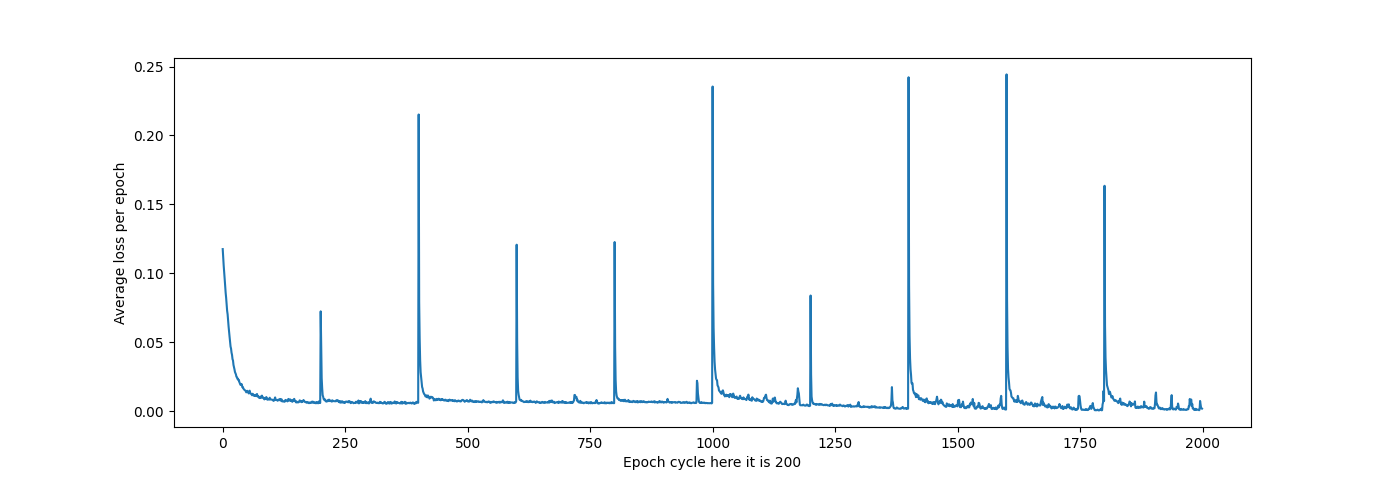
\includegraphics[width=\oneImgWidth]{images/secondAgentTrainChart1}%
    
    \captionadjust%
    \caption{\label{fig:secondAgentTrainChart1} Here is  the training progress for imitating the rulbased agent at the beginning of our second best model.
    }%
\end{figure}

At the beginning of training, our agent aims to imitate the rule-based agent. For this purpose, the ReplayBuffer was filled with data 
from the rule-based agent. After each round, the agent was trained with the current data from the ReplayBuffer. At the start of the training, 
the buffer was relatively empty and had few data points. It took some time to reach a capacity of 500,000. In \autoref{fig:secondAgentTrainChart1}, you can observe 
this (we set \verb|NUM_EPOCH| to 200 here for better visualization). Each time 200 epochs were completed, a new training round began, and the 
ReplayBuffer collected new data. Since the buffer had few data points, new data made up a significant portion, leading to noticeable spikes 
in the loss function at the beginning of each 200-epoch cycle, as seen in \autoref{fig:secondAgentTrainChart1}. This behavior will improve over the course of training, not 
only because the buffer will have more data but also because the agent will learn from it.

In the end, our goal was to eliminate these spikes completely. This indicates that the agent can handle new game states effectively. 
To achieve this, we increased the number of epochs during training and removed old data from the ReplayBuffer. Additionally, we dynamically 
adjusted the batch size. When the buffer had few data points, the batch size was 32, later increased to 512, and eventually set to 1024.
By the way, the training process for the encoder network followed a similar pattern; we simply reduced the dataset size to 100,000. Otherwise, 
the graph looked almost the same, except that the level of the loss function was higher, so it never reached 0.

\begin{figure}[H]
    \centering
    
    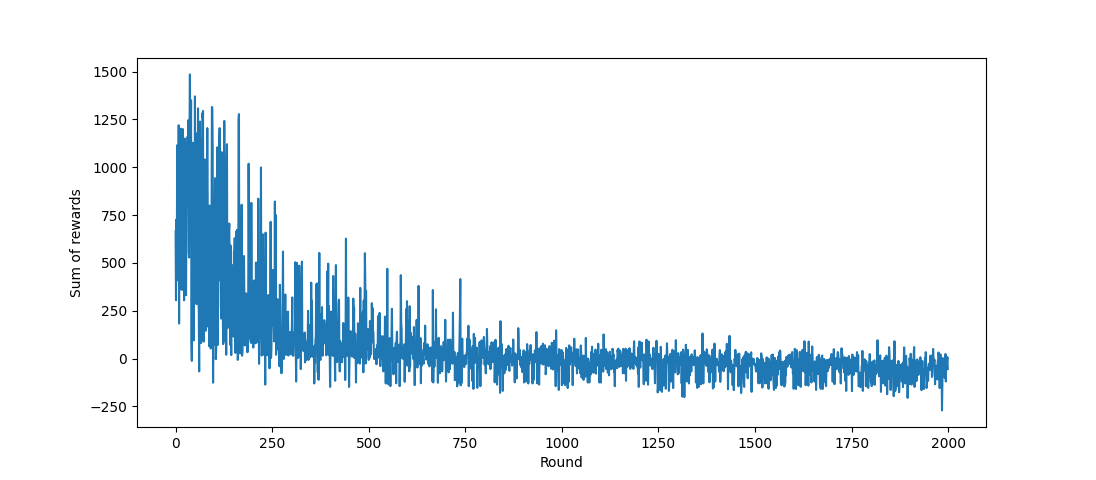
\includegraphics[width=\oneImgWidth]{images/secondAgentTrainChart2}%
    
    \captionadjust%
    \caption{\label{fig:secondAgentTrainChart2} Here is the training progress as we attempted to enhance the agent performance using deep Q-learning.
    }%
\end{figure}

After the agent achieved a decent level of play through training with the rule-based agent, our goal was, of course, 
to further enhance its performance to enable it to defeat other rule-based agents in the game. We thought the agent could 
leverage the knowledge of the rule-based agent and then learn better or different strategies more easily and quickly. 
However, as observed in \autoref{fig:secondAgentTrainChart2}, that was not the case. With increasing training, the agent's performance deteriorated, 
reaching a point where it could no longer play the game. Even when we increased the number of rounds to 20000, there was no improvement. 
We tried various approaches, such as changing the loss function, optimizer, learning rate, and so on, but nothing helped. We suspected that 
one possible reason for this issue was the use of different training sets with labels that were entirely 
differently dimensioned, which might have caused the problem.